\chapter{Appendice A}
\section{CMSIS}
Il CMSIS è uno \textit{standard} software sviluppato da ARM che
fornisce un'interfaccia comune tra l'hardware del core Cortex-M, e i tool software di sviluppo, "Ogni tipo di microcontrollore ha componenti interni 
diversi, ma tutti quelli con un core ARM Cortex-M hanno alcune parti in comune : il SysTick, NVIC ecc\\
ARM ha creato il CMSIS, una specie di manuale standard e libreria di comandi che ti permette di comunicare direttamente con il cuore ARM del microcontrollore in modo uguale per tutti i modelli.

\section{Piastre interdigitate, note anche come \textit{Finger capacitors}}
Le piastre interdigitate sono una configurazione particolare di condensatori utilizzata frequentemente nei sensori MEMS per rilevare spostamenti meccanici con elevata sensibilità.\\
Quando la massa sospesa si sposta a causa di un'accelerazione, cambia la distanza e/o la superficie di sovrapposizione tra le armature mobili e quelle fisse. Poiché la capacità elettrica di un 
condensatore \textit{C} dipende da questi fattori secondo la, semplificata, formula :\\
\begin{equation}
    C = \varepsilon \cdot \frac{\textit{A}}{\textit{d}}
\end{equation}
Dove $\varepsilon$ è la costante dielettrica del materiale tra le piastre, \textit{A} è l'area di sovrapposizione delle piastre, \textit{d} è la distanza tra esse.\\

\begin{figure}[H]
    \centering
    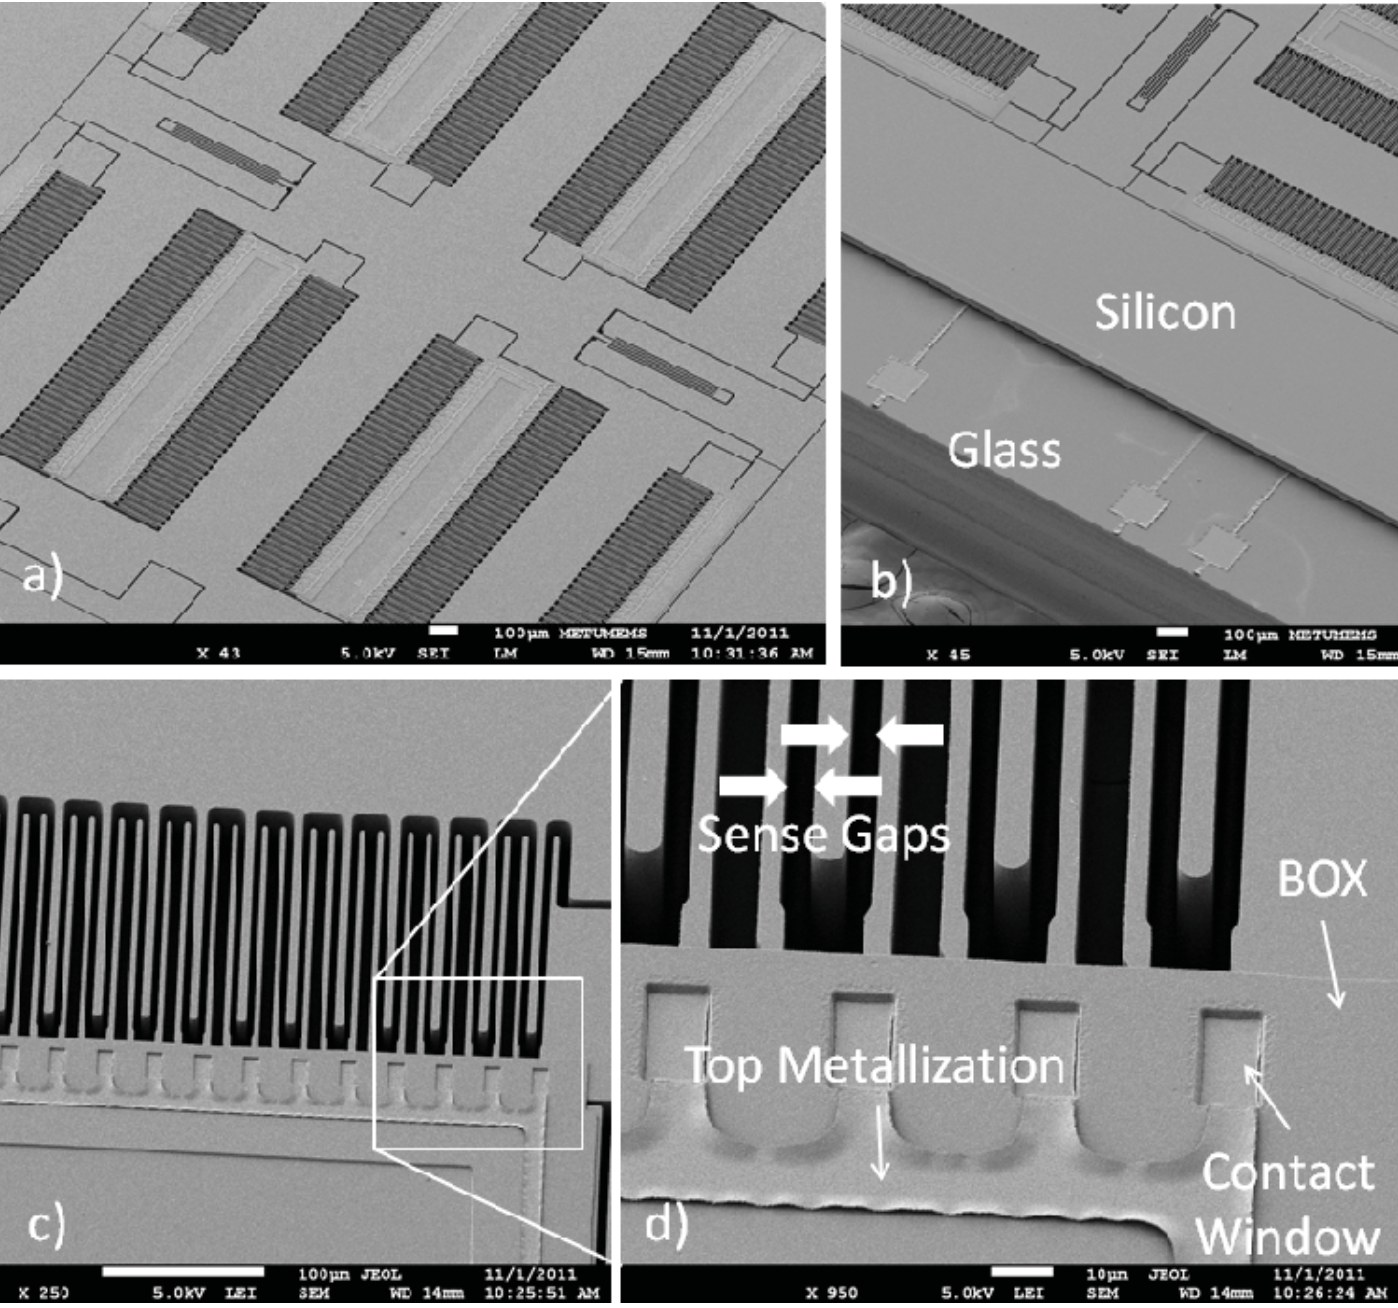
\includegraphics[width = 0.4\textwidth]{images/IMMAGINE_A_1_piastre_inerdigitate .png}
    \caption{Piastre interdigitate}
    \label{fig:etichetta}
\end{figure}